\documentclass[12pt]{report}

% --- Idioma y codificación ---
\usepackage[spanish]{babel}
\usepackage[utf8]{inputenc}

% --- Matemáticas ---
\usepackage{amsmath, amssymb, amsthm}

% --- Gráficos y figuras ---
\usepackage{graphics, graphicx, subfigure}
\usepackage{tikz, pgffor, ifthen}

% --- Tablas y estructuras ---
\usepackage{array, multicol, longtable, booktabs}

% --- Listas y enumeraciones ---
\usepackage{enumerate, enumitem}

% --- Márgenes y geometría ---
\usepackage[a4paper, margin=1.5cm]{geometry}

% --- Diseño y marco ---
\usepackage[framemethod=TikZ]{mdframed}

% --- Texto y contenido de prueba ---
\usepackage{lipsum}

% --- Hipervínculos ---
\usepackage{hyperref}
\hypersetup{
    colorlinks=true,
    linkcolor=black,
    filecolor=magenta,
    urlcolor=cyan
}

% --- Código fuente (listings) ---
\usepackage{listings}
\usepackage{xcolor}
\usepackage{bbm}

\definecolor{listing-background}{HTML}{F7F7F7}
\definecolor{listing-rule}{HTML}{B3B2B3}
\definecolor{listing-numbers}{HTML}{B3B2B3}
\definecolor{listing-text-color}{HTML}{000000}
\definecolor{listing-keyword}{HTML}{435489}
\definecolor{listing-keyword-2}{HTML}{1284CA}
\definecolor{listing-keyword-3}{HTML}{9137CB}
\definecolor{listing-identifier}{HTML}{435489}
\definecolor{listing-string}{HTML}{00999A}
\definecolor{listing-comment}{HTML}{8E8E8E}

\lstdefinestyle{myStyle}{
    language=C++,
    alsolanguage=scala,
    numbers=left,
    xleftmargin=2.7em,
    framexleftmargin=2.5em,
    backgroundcolor=\color{gray!15},
    basicstyle=\color{listing-text-color}\linespread{1.0}\ttfamily,
    breaklines=true,
    frameshape={RYR}{Y}{Y}{RYR},
    rulecolor=\color{black},
    tabsize=2,
    numberstyle=\color{listing-numbers}\linespread{1.0}\small\ttfamily,
    aboveskip=1.0em,
    belowskip=0.1em,
    abovecaptionskip=0em,
    belowcaptionskip=1.0em,
    keywordstyle={\color{listing-keyword}\bfseries},
    keywordstyle={[2]\color{listing-keyword-2}\bfseries},
    keywordstyle={[3]\color{listing-keyword-3}\bfseries\itshape},
    sensitive=true,
    identifierstyle=\color{listing-identifier},
    commentstyle=\color{listing-comment},
    stringstyle=\color{listing-string},
    showstringspaces=false,
    label=lst:bar,
    captionpos=b
}
\lstset{style=myStyle}

% --- Marca de agua ---
\usepackage{eso-pic}
\AddToHook{shipout/foreground}{
    \begin{tikzpicture}[remember picture,overlay]
        \node at (current page.center){
            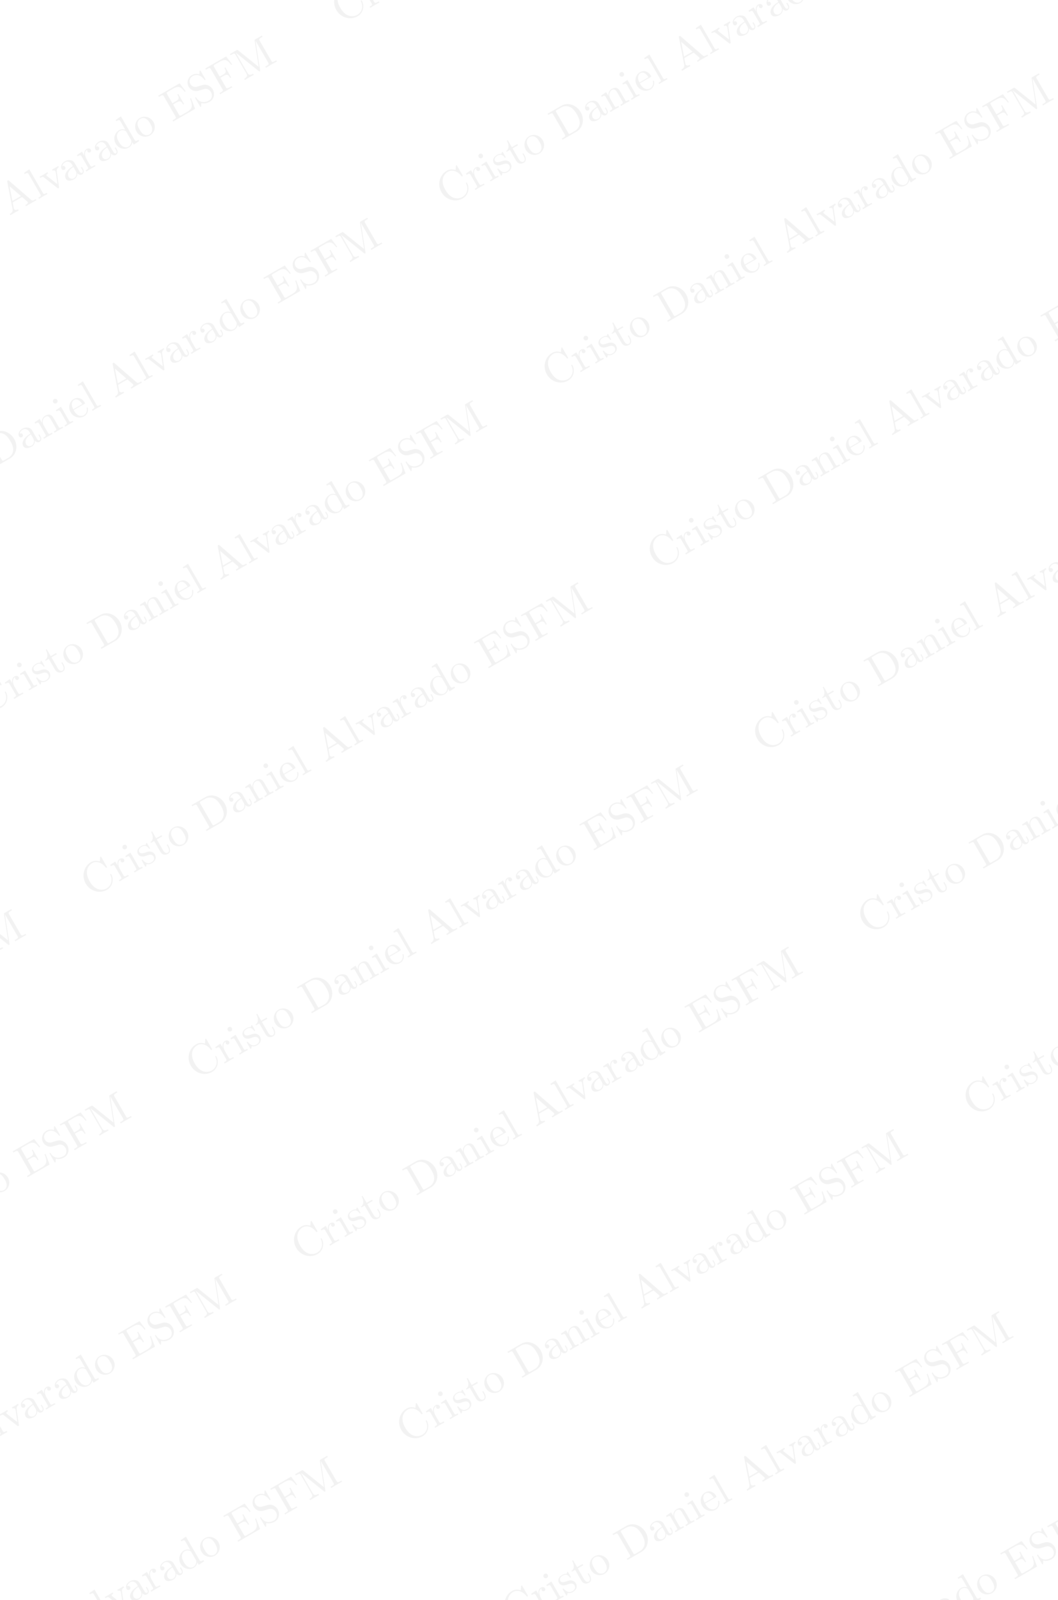
\includegraphics[width=\paperwidth,height=\paperheight,keepaspectratio]{watermark-1.png}
        };
    \end{tikzpicture}
}

% --- Redefinición de encabezados de capítulo ---
\makeatletter
\def\@makechapterhead#1{%
  {\parindent \z@ \raggedright
    \reset@font
    \hrule
    \vspace*{10\p@}
    \par
    \center \LARGE \scshape \@chapapp{} \huge \thechapter
    \vspace*{10\p@}
    \par\nobreak
    \vspace*{10\p@}
    \par
    \vspace*{1\p@}
    \hrule
    \vspace*{60\p@}
    \Huge #1\par\nobreak
    \vskip 50\p@
  }}
\makeatother

% --- Entornos personalizados ---
% (aquí puedes definir tus theorems, definiciones, etc.)


% --- Entornos personalizados ---
\newtheoremstyle{largebreak}{}{ }{\normalfont}{}{\bfseries}{}{\newline}{}
\theoremstyle{largebreak}

\newmdtheoremenv[hidealllines=true,roundcorner=5pt,backgroundcolor=gray!60!red!30]{exa}{Ejemplo}[section]
\newmdtheoremenv[hidealllines=true,roundcorner=5pt,backgroundcolor=gray!50!blue!30]{obs}{Observaci\'on}[section]
\newmdtheoremenv[hidealllines=true,roundcorner=5pt,backgroundcolor=green!50!blue!30]{preg}{Pregunta}[section]
\newmdtheoremenv[hidealllines=true,roundcorner=5pt,backgroundcolor=yellow!40]{idea}{Idea}[section]
\newmdtheoremenv[rightline=false,leftline=false]{theor}{Teorema}[section]
\newmdtheoremenv[rightline=false,leftline=false]{propo}{Proposici\'on}[section]
\newmdtheoremenv[rightline=false,leftline=false]{cor}{Corolario}[section]
\newmdtheoremenv[rightline=false,leftline=false]{lema}{Lema}[section]
\newmdtheoremenv[roundcorner=5pt,backgroundcolor=gray!30,hidealllines=true]{mydef}{Definici\'on}[section]
\newmdtheoremenv[roundcorner=5pt]{excer}{Ejercicio}[section]

% --- Comandos auxiliares ---
\def\proof{\paragraph{Demostraci\'on:\\}}
\def\endproof{\hfill$\blacksquare$}
\def\sol{\paragraph{Soluci\'on:\\}}
\def\endsol{\hfill$\square$}

\newcommand\abs[1]{\ensuremath{\left|#1\right|}}
\newcommand\divides{\ensuremath{\bigm|}}
\newcommand\cf[3]{\ensuremath{#1:#2\rightarrow#3}}
\newcommand\contradiction{\ensuremath{\#_c}}
\newcommand\natint[1]{\ensuremath{\left[\big|#1\big|\right]}}
\newcommand{\bbm}[1]{\mathbbm{#1}}
\newcommand{\pot}[1]{\mathcal{P}\left(#1\right)}
\newcommand{\Prob}[1]{\mathbbm{P}\left(#1\right)}

\newcounter{figcount}
\setcounter{figcount}{1}

\renewcommand{\lstlistingname}{Código}
\renewcommand{\lstlistlistingname}{Lista de \lstlistingname s}

% --- Comienzo del documento ---
\begin{document}

    \setlength{\parskip}{5pt}
    \setlength{\parindent}{12pt}
    \title{Probability Notes}
    \author{Cristo Daniel Alvarado}
    \maketitle

    \tableofcontents

    \newpage

    \chapter{Basic Probability}

    This document aims to cover the basics of probability in a simplified and straightforward way. Occasionally, exercises are included to illustrate the use of certain theorems, propositions, lemmas, and definitions that are presented. The goal is to later move on to inferential statistics, rather than focusing on elementary probability.

    It may be possible that as time goes by, the notes are extended to cover a larger amount of content that aims the study of probability as an independent subject of statistics.

    \section{Fundations}

    \begin{mydef}[\textbf{Sample Space}]
        Let $\Omega$ be a set. We say that $\Omega$ is a \textbf{sample space} if is the set of possible outcomes of an experiment. Points in $\Omega$ are called sample \textbf{outcomes}, \textbf{realizations} or \textbf{elements}.

        If $\Gamma\subseteq\Omega$, then $\Gamma$ is called an \textbf{event}.
    \end{mydef}

    \begin{exa}[\textbf{Example of a Sample Space}]
        If we toss a coin forever, the sample space of the experiment is the set:
        \begin{equation*}
            \Omega=\left\{\cf{\omega}{\bbm{N}}{\left\{H,T\right\}}\Big|\omega\textup{ is a function} \right\},
        \end{equation*}
        where $\left\{H,T\right\}$ represents the positions of Heads and Tails, respectively. Let $E$ be an event such that:
        \begin{itemize}
            \item The first head appears on the third toss, then:
            \begin{equation*}
                E=\left\{\omega\in\Omega\Big| \omega(1)=\omega(2)=T\textup{ and }\omega(3)=H\right\}.
            \end{equation*}
        \end{itemize}
    \end{exa}

    \begin{obs}[\textbf{Complement of an Event}]
        Given an event $E$ in a sample space $\Omega$, we denote by $E^c$ its complement relative to $\Omega$, that is:
        \begin{equation*}
            E^c=\Omega\setminus E=\left\{\omega\in\Omega\Big|\omega\notin E \right\}
        \end{equation*}
    \end{obs}

    The event $\emptyset$ is called the \textbf{null event} and $\Omega$ is called the \textbf{true event}.

    \begin{mydef}[\textbf{Indicator Function}]
        Let $\Omega$ be a sample space. If $A$ is an event of $\Omega$, then we define it's \textbf{indicator function}, denoted by $\bbm{1}_A$ such that:
        \begin{equation*}
            \bbm{1}_A(\omega)=\left\{
                \begin{array}{lcr}
                    1 & \textup{ if } & \omega\in A\\
                    0 & \textup{ if } & \omega\notin A\\
                \end{array}
            \right.,\quad\forall\omega\in\Omega.
        \end{equation*}
    \end{mydef}

    Let $\Omega$ be a sample space. We introduce a partial order in the set $\pot{\Omega}$ (where $\pot{\Omega}$ is the power set of $\Omega$) as follows:
    \begin{equation*}
        A_1\subseteq A_2\iff \omega\in A_2,\quad\forall \omega\in A_1
    \end{equation*}
    that is, this is the inclusion relation restricted to the set $\pot{\Omega}$.

    \begin{mydef}[\textbf{Sequence of Monotone Increasing and Decreasing Events}]
        Let $\Omega$ be a sample space. A sequence of events $\left(A_n\right)_{ n=1}^\infty$ is:
        \begin{itemize}
            \item \textbf{Monotone increasing} if $A_i\subseteq A_{i+1}$, for all $i\in\mathbb{N}$.
            \item \textbf{Monotone decreasing} if $A_{i+1}\subseteq A_i$, for all $i\in\mathbb{N}$.
        \end{itemize}
    \end{mydef}

    Obviously, we can generalize the latter definition by just stating that $\left(A_n\right)_{ n=1}^\infty$ is a sequence of sets. Right now we'll be working only with sample spaces, so no further explanation is required.

    From now on, $\Omega$ will be a set and it'll always be a sample space.

    \section{Mesures}

    If $A$ is an event on a sample space $\Omega$, we want to somehow assign this event a real number called its probability. We do this with the following definition:

    \begin{mydef}[\textbf{Probability Measure or Distribution}]
        Let $\Omega$ be a sample space. A function $\cf{\bbm{P}}{\pot{\Omega}}{\bbm{R}}$ is a \textbf{probability distribution} or \textbf{probability measure} if it satisfies the following:
        \begin{enumerate}[label = \textit{(\arabic*)}]
            \item $\Prob{A}\geq 0$, for all $A\subseteq\Omega$.
            \item $\Prob{\Omega}=1$.
            \item If $\left(A_n\right)_{ n=1}^\infty$ is a sequence of disjoint events, then:
            \begin{equation*}
                \Prob{\bigcup_{ n=1}^\infty A_n}=\sum_{ n=1}^\infty\Prob{A_n}
            \end{equation*}
        \end{enumerate}
    \end{mydef}

    \begin{obs}
        It will not be always possible to assign a probability to every event in a sample space. This happens (for example) in the real line. If we want certain properties of the real line to be satisfied, it will be impossible to assign a probability to each event of our sample space.
    \end{obs}

\end{document}